\documentclass[border = 10pt]{standalone}
\RequirePackage{pgf,pgffor}
\usepackage{tikz}
\usetikzlibrary{arrows, shapes.gates.logic.US, calc}
\usetikzlibrary{circuits.ee.IEC}
\usepgflibrary{shapes.gates.logic} % LATEX and plain TEX and pure pgf 
%\usepgflibrary[shapes.gates.logic] % ConTEXt and pure pgf 
%\usetikzlibrary{shapes.gates.logic} % LATEX and plain TEX when using TikZ 
%\usetikzlibrary{shapes.gates.logic} % ConTEXt when using TikZ
\begin{document}

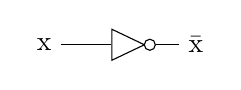
\begin{tikzpicture}
    \node[not gate US, draw, rotate=0, logic gate inputs=n] at (0,0) (notg) {};
    \node (x) at (-1,0) {x};
    \draw (x) -- (notg.input);
    \draw (notg.output) -- node[right,fill=white]{$\bar{\textrm{x}}$}(1,0);
\end{tikzpicture}

\end{document}